\section{证据一：多跳外推与三阶段泛化}
\label{sec:grokking-evidence}

本章的结论是：视频给出的多跳外推和三阶段泛化证据，说明递归深度可能形成可复用的计算过程。这个证据有技术价值，也需要严格限界。它支持“循环次数可以成为测试时计算旋钮”这一判断；它尚不足以推出循环 Transformer 已经拥有通用推理优势。

\begin{importantbox}{本章主张}
行为证据的核心意义在于：当推理时增加循环次数，模型有机会处理比训练阶段更长的关系链。若这种外推稳定出现，递归模块除节省参数外，还可能学到可重复调用的推理更新规则。
\end{importantbox}

\subsection{《Loop, Think, and Generalize》的证据入口}

视频在 00:05:40 之后提到《Loop, Think, and Generalize》，并把它作为 Loop Transformer 行为证据的入口。讲义应把这里写成“视频中的论文叙述”：循环架构在多跳推理任务上表现更好，并且当推理阶段增加循环迭代时，模型能够处理超过训练深度的跳数。

这个现象如果成立，含义很重要。模型训练时只见过较短的跳数，推理时却能通过更多循环处理更长链条，说明它可能学到了一种“重复应用的关系更新规则”。类比到查资料：训练时只练过“查两次索引”，测试时增加循环次数后可以查三次、四次；关键能力在于每次查到中间结果后，仍能把它转成下一次查询的有效状态。

\subsection{三阶段 Grokking：从记忆到系统化组合}

视频画面中的三阶段顿悟式泛化（grokking）曲线把训练过程分成三个阶段：记忆训练样本、分布内泛化、系统化泛化。它的教学价值在于让读者看到，模型能力提升可能呈现阶梯式打开，偏离“平滑多记一点”的朴素想象。

\begin{figure}[htbp]
    \centering
    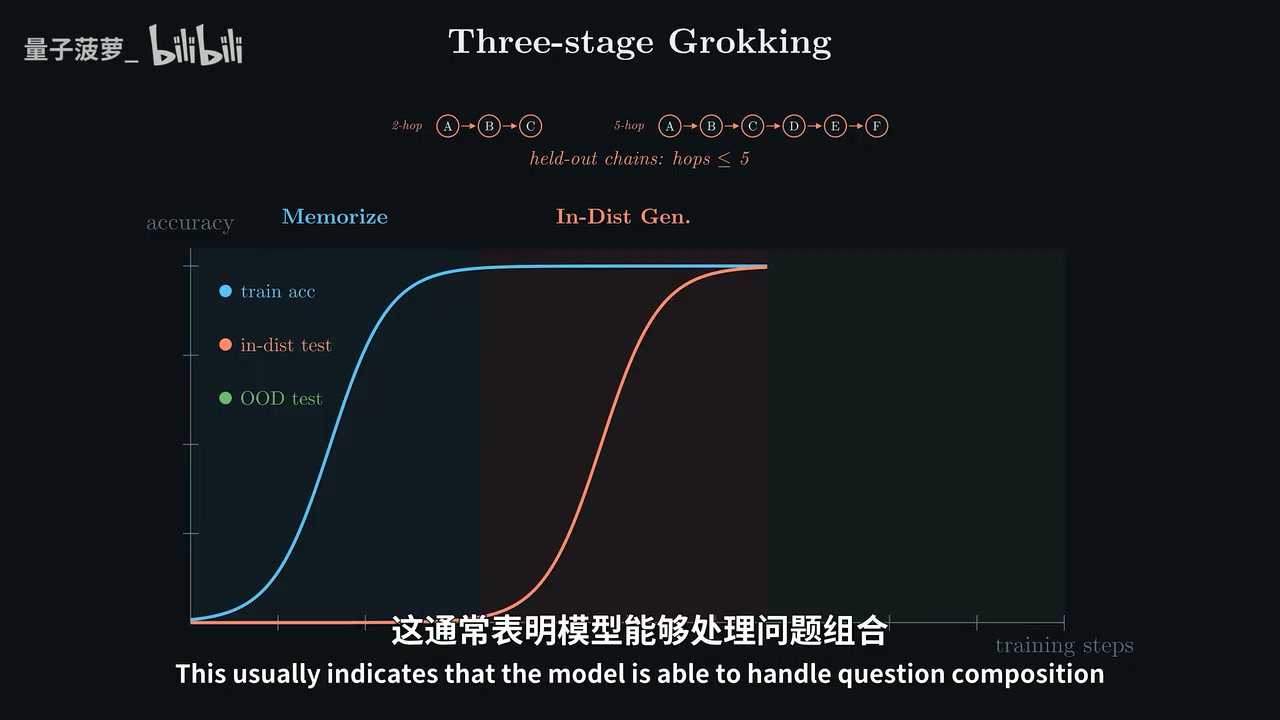
\includegraphics[width=0.82\linewidth,height=0.36\textheight,keepaspectratio]{figures/fig_06_three_stage_grokking.jpg}
    \caption{三阶段 grokking 曲线：训练准确率先上升，随后分布内测试提升，最后才出现面向未见组合的系统化泛化。\protect\footnotemark}
    \label{fig:grokking-three-stages}
\end{figure}
\footnotetext{视频画面时间区间：00:06:00--00:06:24。}

第一阶段是记忆（memorization）。蓝色训练准确率先上升，表示模型逐渐掌握训练样本中的具体链条。这个阶段像背题：给定熟悉组合，模型能够答对。

第二阶段是分布内泛化（in-distribution generalization）。橙色测试曲线随后上升，表示模型开始处理与训练结构相同、具体样本不同的问题。这个阶段像学会同一类题的解法：题目换了，规则仍相近。

第三阶段是系统化泛化（systematic generalization）。视频把它描述为模型能够组合训练期间未组合过的知识片段，也就是对分布外（out-of-distribution, OOD）组合的处理能力增强。这个阶段最接近“学会规则”：模型不只复述见过的路径，还能把局部关系重新拼接成新的答案链。

\begin{knowledgebox}{为什么 grokking 容易被误读}
Grokking 常被理解为“模型突然开窍”。更严格的说法是：不同评测集合上的准确率在训练过程中先后跨过阈值。它展示的是行为曲线的阶段性变化；若要证明内部算法，还需要后续的机制分析，例如隐藏状态轨迹、固定点、注意力头行为等证据。
\end{knowledgebox}

\subsection{递归深度作为测试时计算旋钮}

视频在 00:06:47 之后强调：当推理时增加循环次数，模型可以完成比训练时更多的跳跃。在 Loop Transformer 中，递归次数 \(R\) 就成为一种计算调节器。普通 CoT 通过生成更多 token 增加计算；循环模型通过增加内部递归步增加计算。

先用普通话解释这个公式：若训练时模型主要使用 \(R_{\mathrm{train}}\) 次循环，推理时把循环次数提高到 \(R_{\mathrm{test}}\)，模型就在更长的状态更新链上应用同一个规则。计算量会随递归次数增加而增加，收益取决于这个更新规则是否能稳定外推。

$$
R_{\mathrm{test}}>R_{\mathrm{train}},\qquad C_{\mathrm{loop}}\propto R_{\mathrm{test}}
$$

符号说明如下：
\begin{itemize}
    \item \(R_{\mathrm{train}}\)：训练阶段使用或主要暴露给模型的递归次数。
    \item \(R_{\mathrm{test}}\)：推理阶段实际运行的递归次数。
    \item \(C_{\mathrm{loop}}\)：循环推理的近似计算成本。
    \item \(\propto\)：正比关系，用于表达“递归次数越多，计算成本越高”的一阶直觉。
\end{itemize}

这个公式的价值在于把“更长时间思考”落到可调参数上。CoT 的旋钮是 token 数和采样路径；Loop Transformer 的旋钮是递归深度。两者都属于测试时计算，只是一个发生在文本序列中，一个发生在隐藏状态中。

\subsection{证据边界：有力线索与过度外推之间}

本章必须谨慎。多跳表现提升和超过训练深度的外推，是支持循环架构的有力线索；它们还只能说明“递归深度可能形成可复用计算过程”。若把它直接写成“循环 Transformer 已经证明通用推理能力更强”，证据链会过长。

\begin{warningbox}{证据边界}
受控多跳任务能检验关系链追踪、状态保持和组合泛化。真实大规模推理还包含噪声上下文、开放世界知识、工具调用、长程依赖、训练分布偏差和系统延迟约束。三阶段曲线说明了值得继续研究的方向，尚需和机制分析、稳定性、缓存成本以及真实任务评测共同判断。
\end{warningbox}

因此，本章与第二章之间的关系应当这样理解：第二章定义了递归机制，第三章说明这种机制可能带来行为收益。后续章节还需要回答两个硬问题：重复应用同一模块是否稳定，以及隐藏状态里发生的变化是否可观察、可解释、可监督。

\subsection{本章小结}

本章从视频中的《Loop, Think, and Generalize》叙述出发，解释了三阶段 grokking 与多跳外推的意义。记忆阶段说明模型先掌握训练样本；分布内泛化说明模型开始处理同结构新题；系统化泛化说明模型可能学到可组合的关系更新规则。递归深度 \(R\) 因此成为测试时计算旋钮：增加循环次数可以给模型更多内部更新机会。结论需要克制：这些行为证据支持“递归可能学到可复用计算过程”，后文仍需检查稳定性、机制可解释性和工程边界。
